\documentclass[xetex,mathserif,serif]{beamer}
\usepackage{polyglossia}
\usepackage{minted}
\usepackage{tabu}

\usepackage{textpos}
\setlength{\TPHorizModule}{1cm}
\setlength{\TPVertModule}{1cm}

\useoutertheme{infolines}

\usepackage{fontspec}
\setmainfont{FreeSans}
\newfontfamily{\russianfonttt}{FreeSans}

\setbeamertemplate{blocks}[rounded][shadow=false]
\setbeamercolor*{block title example}{fg=green!50!black,bg=green!20}
\setbeamercolor*{block body example}{fg=black,bg=green!10}

\setbeamercolor*{block title alerted}{fg=red!50!black,bg=red!20}
\setbeamercolor*{block body alerted}{fg=black,bg=red!10}

\definecolor{cadmiumgreen}{rgb}{0.0, 0.42, 0.24}

\tabulinesep=0.7mm

\title{Обзор LASER-2017}
\author[Юрий Литвинов]{Ю.В. Литвинов \newline 
	А.Н. Терехов \newline
	\textcolor{gray}{\small\texttt{y.litvinov@spbu.ru}} \newline
	\textcolor{gray}{\small\texttt{a.terekhov@spbu.ru}}
}

\date{29.09.2017}

\begin{document}

	\frame{\titlepage}

	\section{Введение}

	\begin{frame}
		\frametitle{LASER-2017}
		\begin{itemize}
			\item Летняя школа, с 9 по 17 сентября, о. Эльба, Италия
			\item Тема школы этого года: \textbf{Software for Robotics}
			\item Формат: 7 лекций по 45 минут в день + студенческие презентации
			\item 7 докладчиков, примерно по 6 лекций на каждого:
			\begin{itemize}
				\item Davide Brugali, University of Bergamo
				\item Rodolphe Gelin, Softbank Robotics
				\item Ashish Kapoor, Microsoft Research
				\item Nenad Medvidovic, University of Southern California
				\item Bertrand Meyer, Politecnico di Milano
				\item Issa Nesnas, NASA Jet Propulsion Laboratory
				\item Hiroshi ``Gitchang'' Okuno, Waseda University and Kyoto University
			\end{itemize}
		\end{itemize}
	\end{frame}

	\section{D. Brugali}

	\begin{frame}
		\begin{center}
			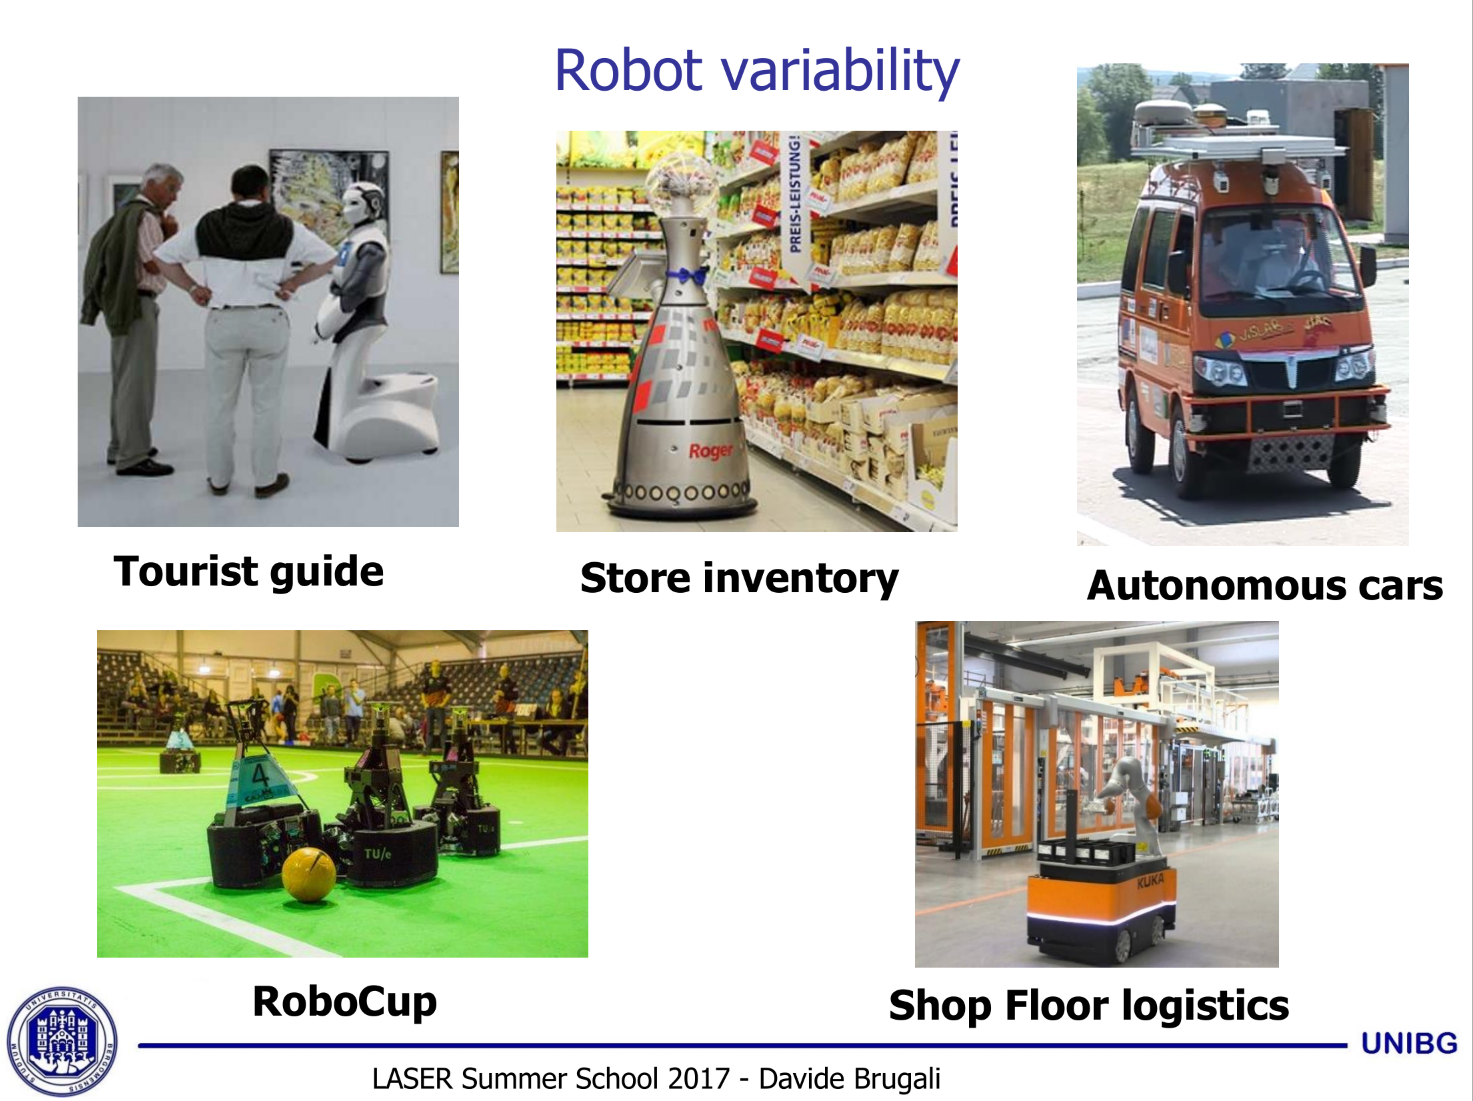
\includegraphics[width=0.9\textwidth]{brugali1.png}
		\end{center}
	\end{frame}

	\begin{frame}
		\begin{center}
			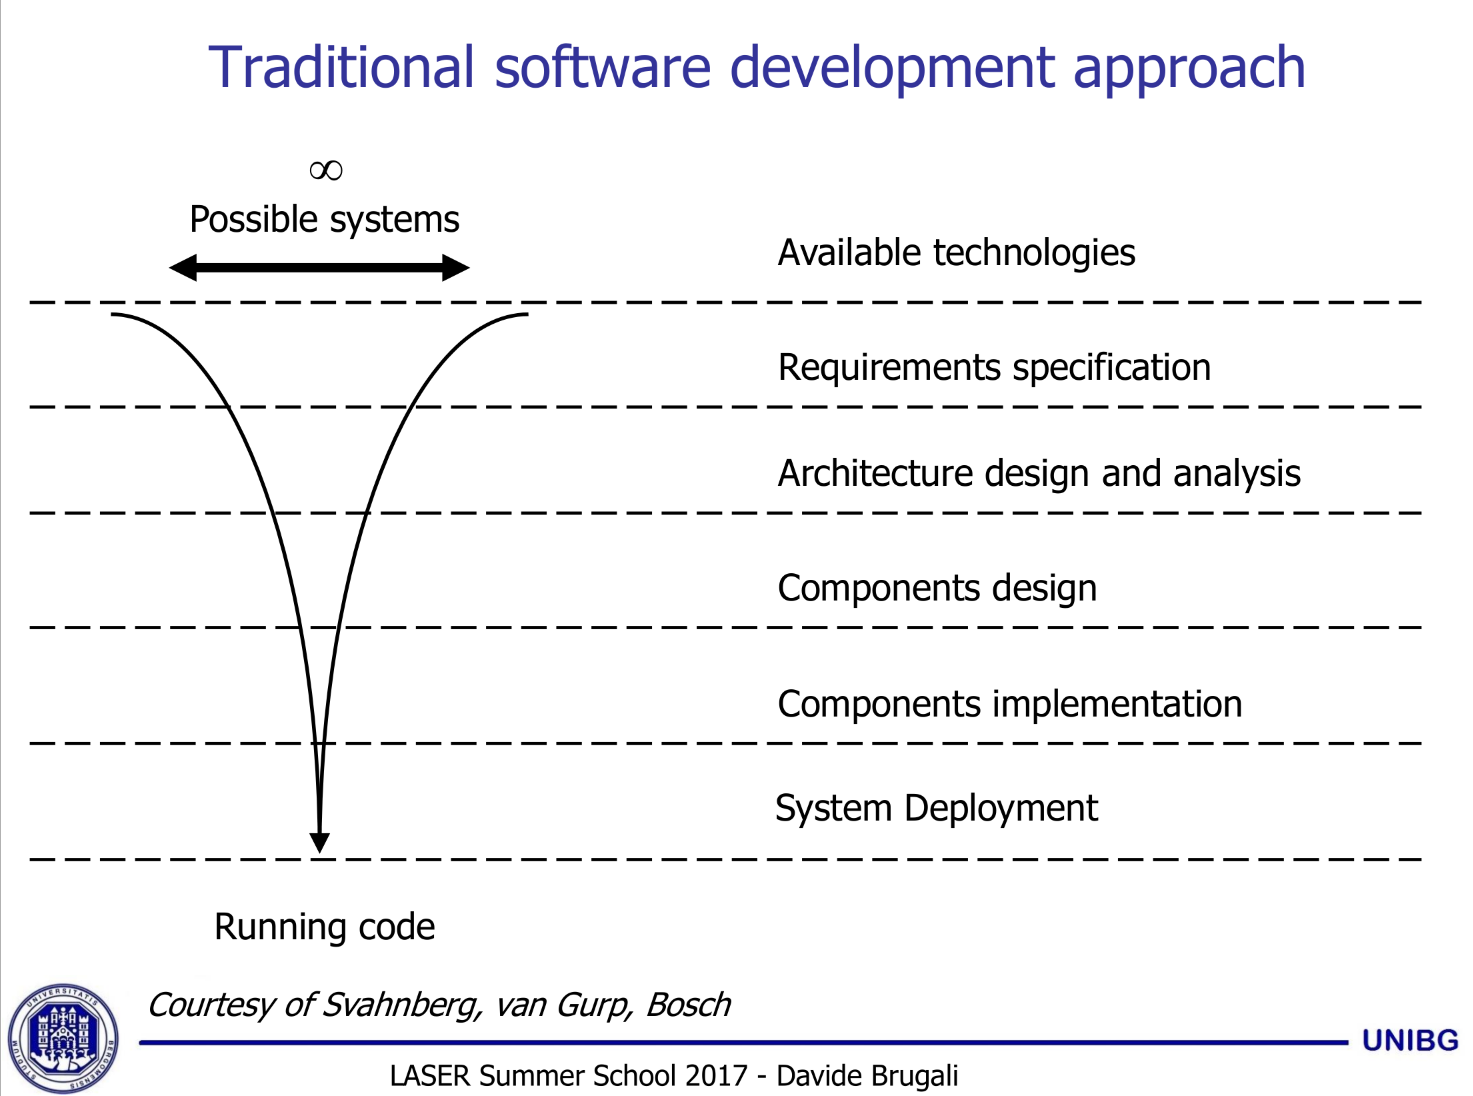
\includegraphics[width=0.9\textwidth]{brugali2.png}
		\end{center}
	\end{frame}

	\begin{frame}
		\begin{center}
			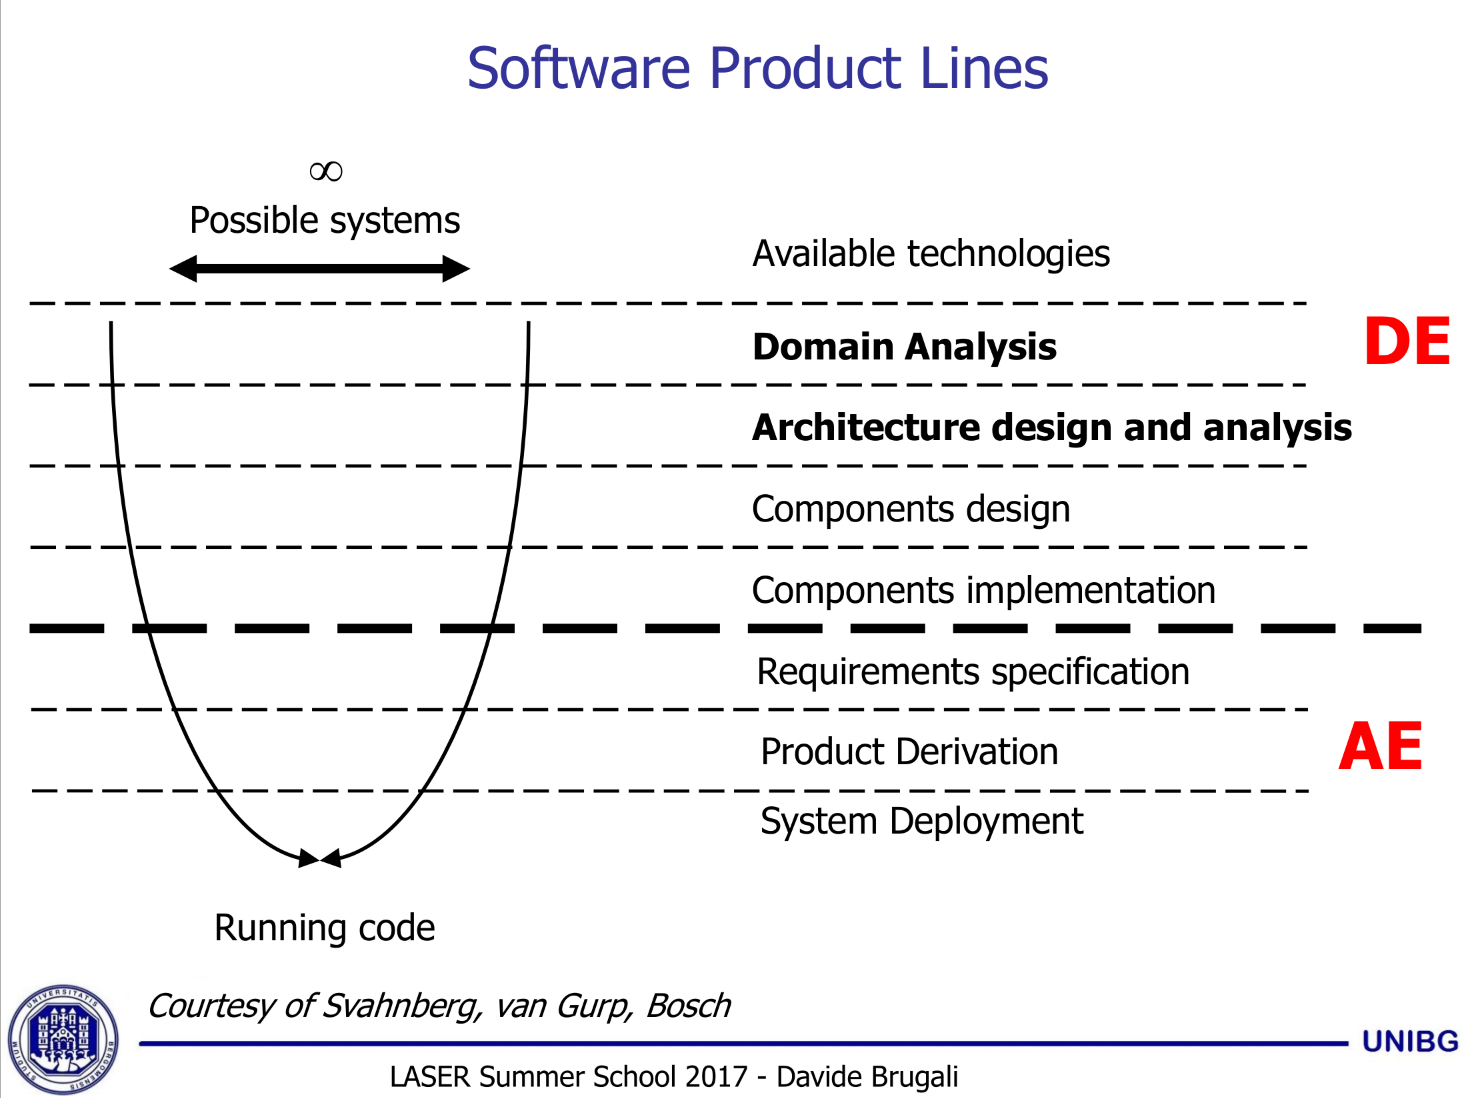
\includegraphics[width=0.9\textwidth]{brugali3.png}
		\end{center}
	\end{frame}

	\begin{frame}
		\begin{center}
			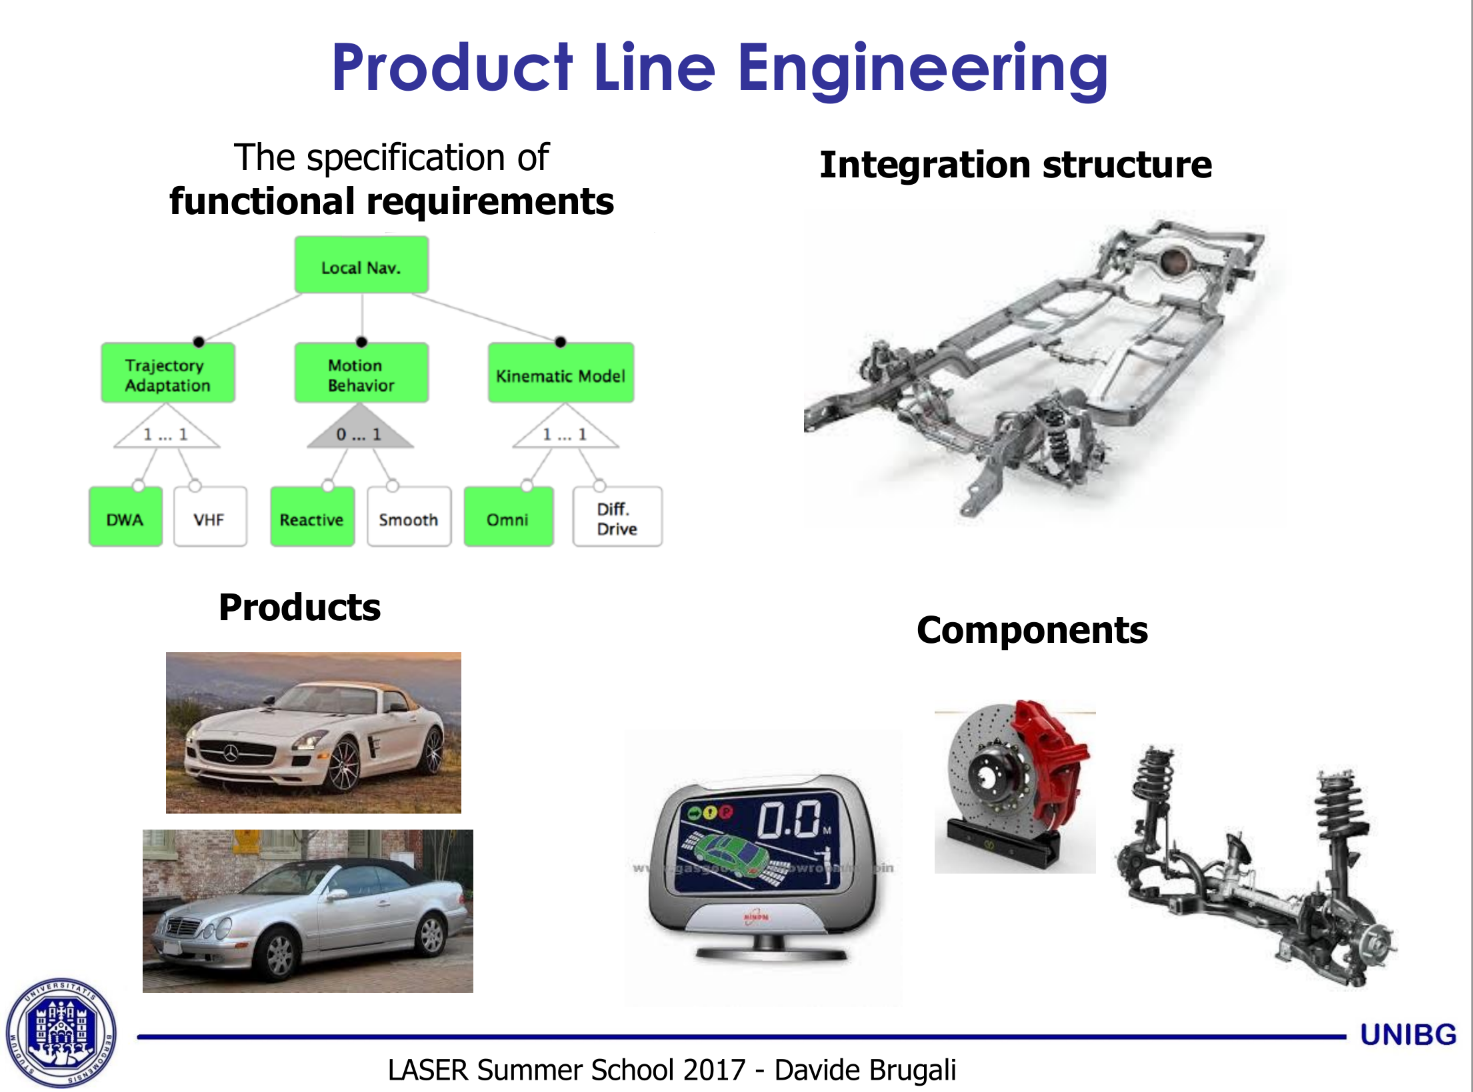
\includegraphics[width=0.9\textwidth]{brugali4.png}
		\end{center}
	\end{frame}

	\begin{frame}
		\begin{center}
			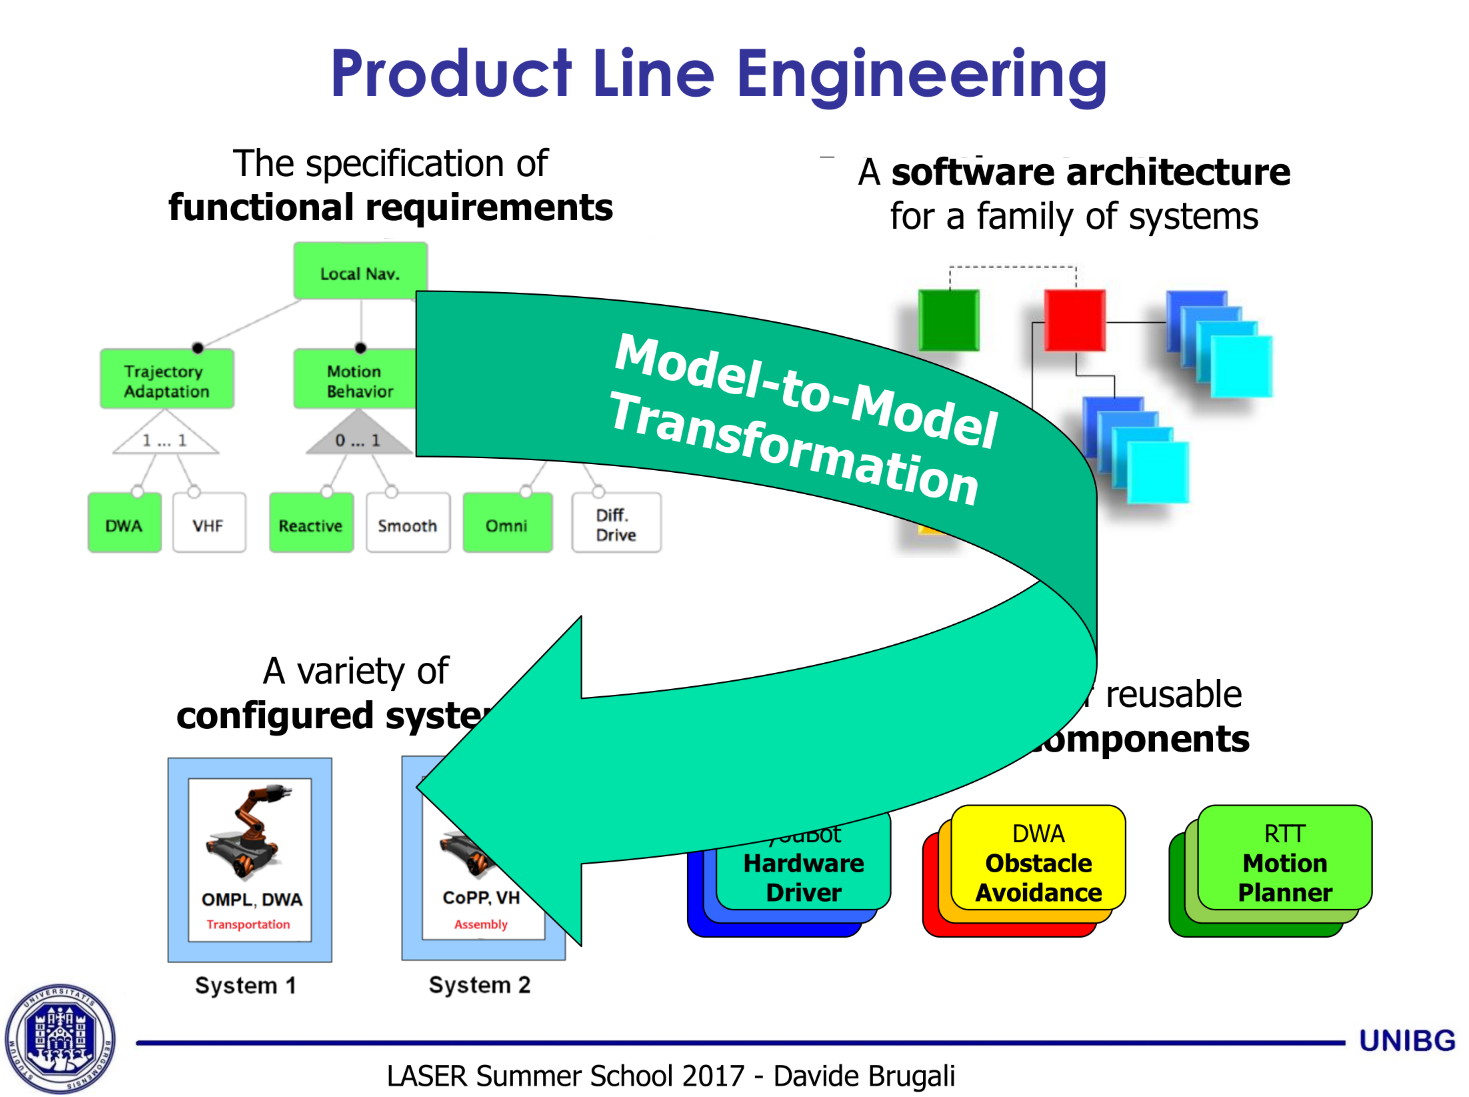
\includegraphics[width=0.9\textwidth]{brugali5.png}
		\end{center}
	\end{frame}

	\begin{frame}
		\begin{center}
			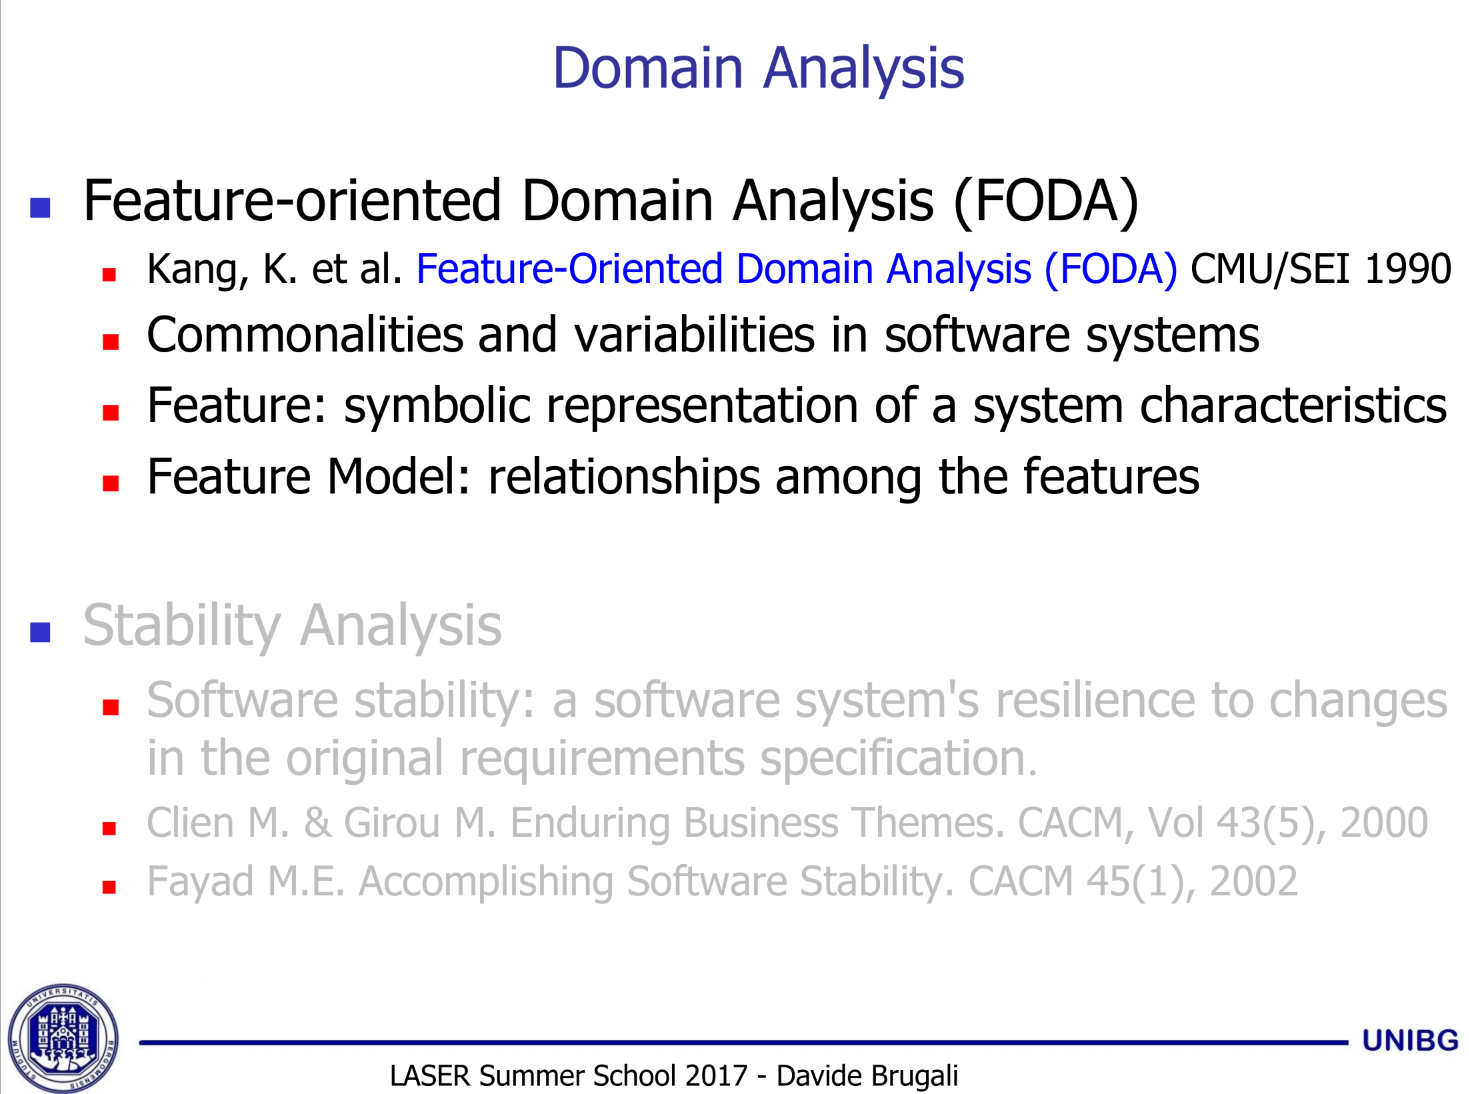
\includegraphics[width=0.9\textwidth]{brugali6.png}
		\end{center}
	\end{frame}

	\begin{frame}
		\begin{center}
			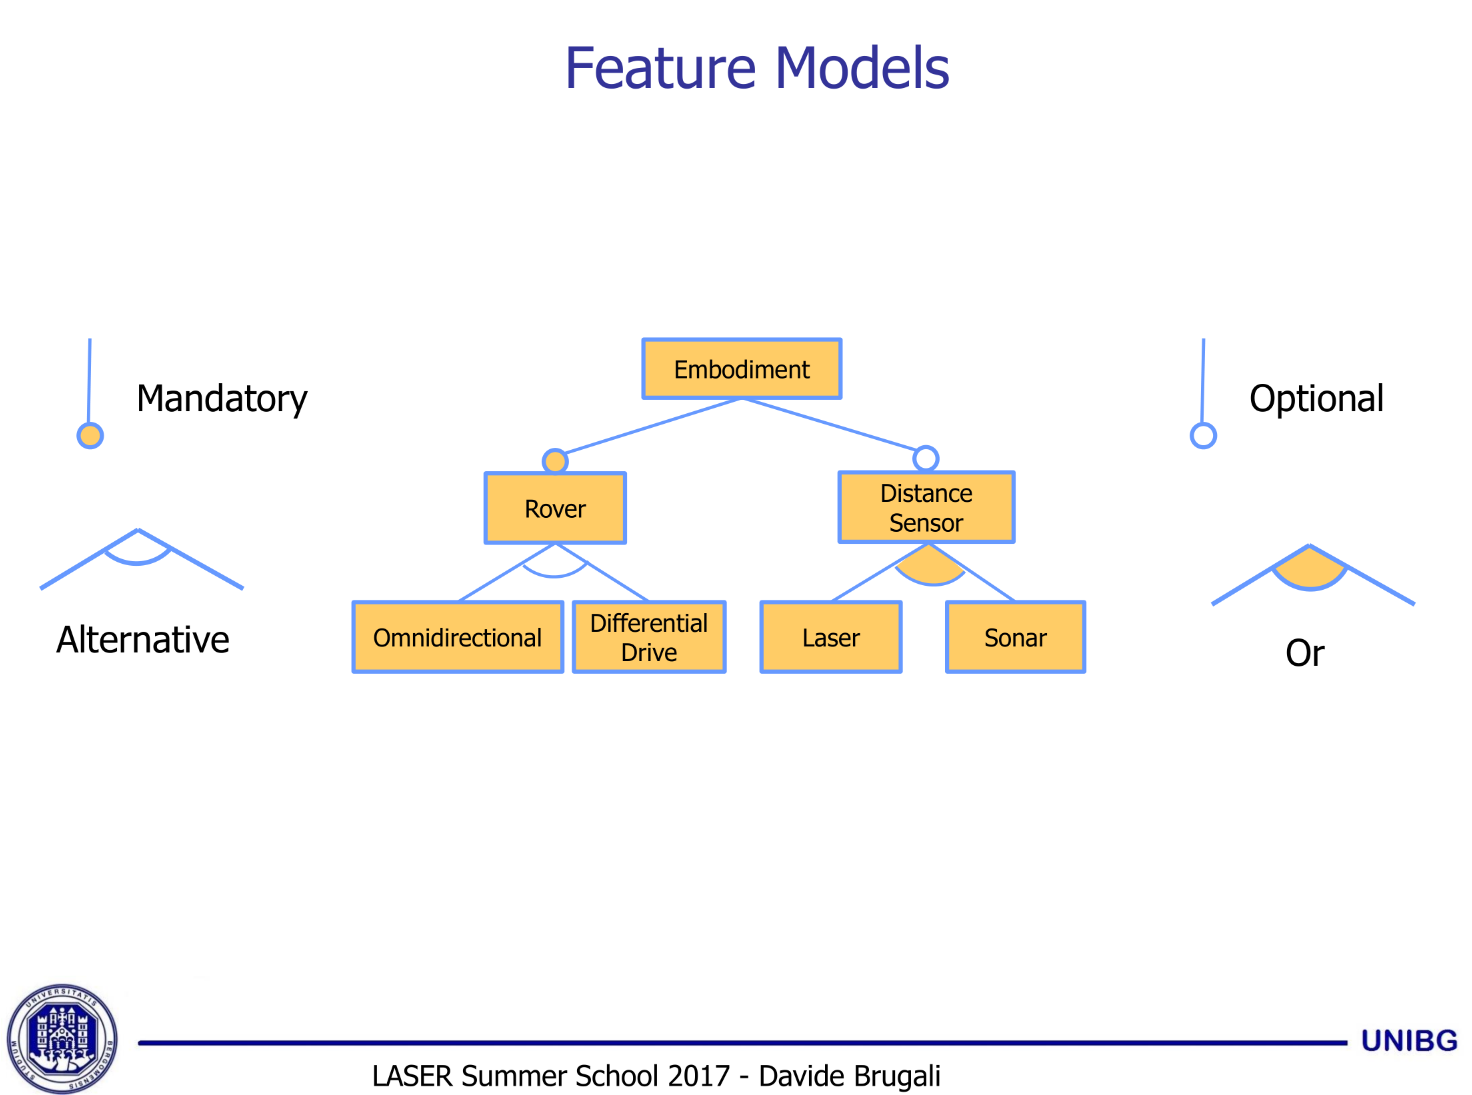
\includegraphics[width=0.9\textwidth]{brugali7.png}
		\end{center}
	\end{frame}

	\begin{frame}
		\begin{center}
			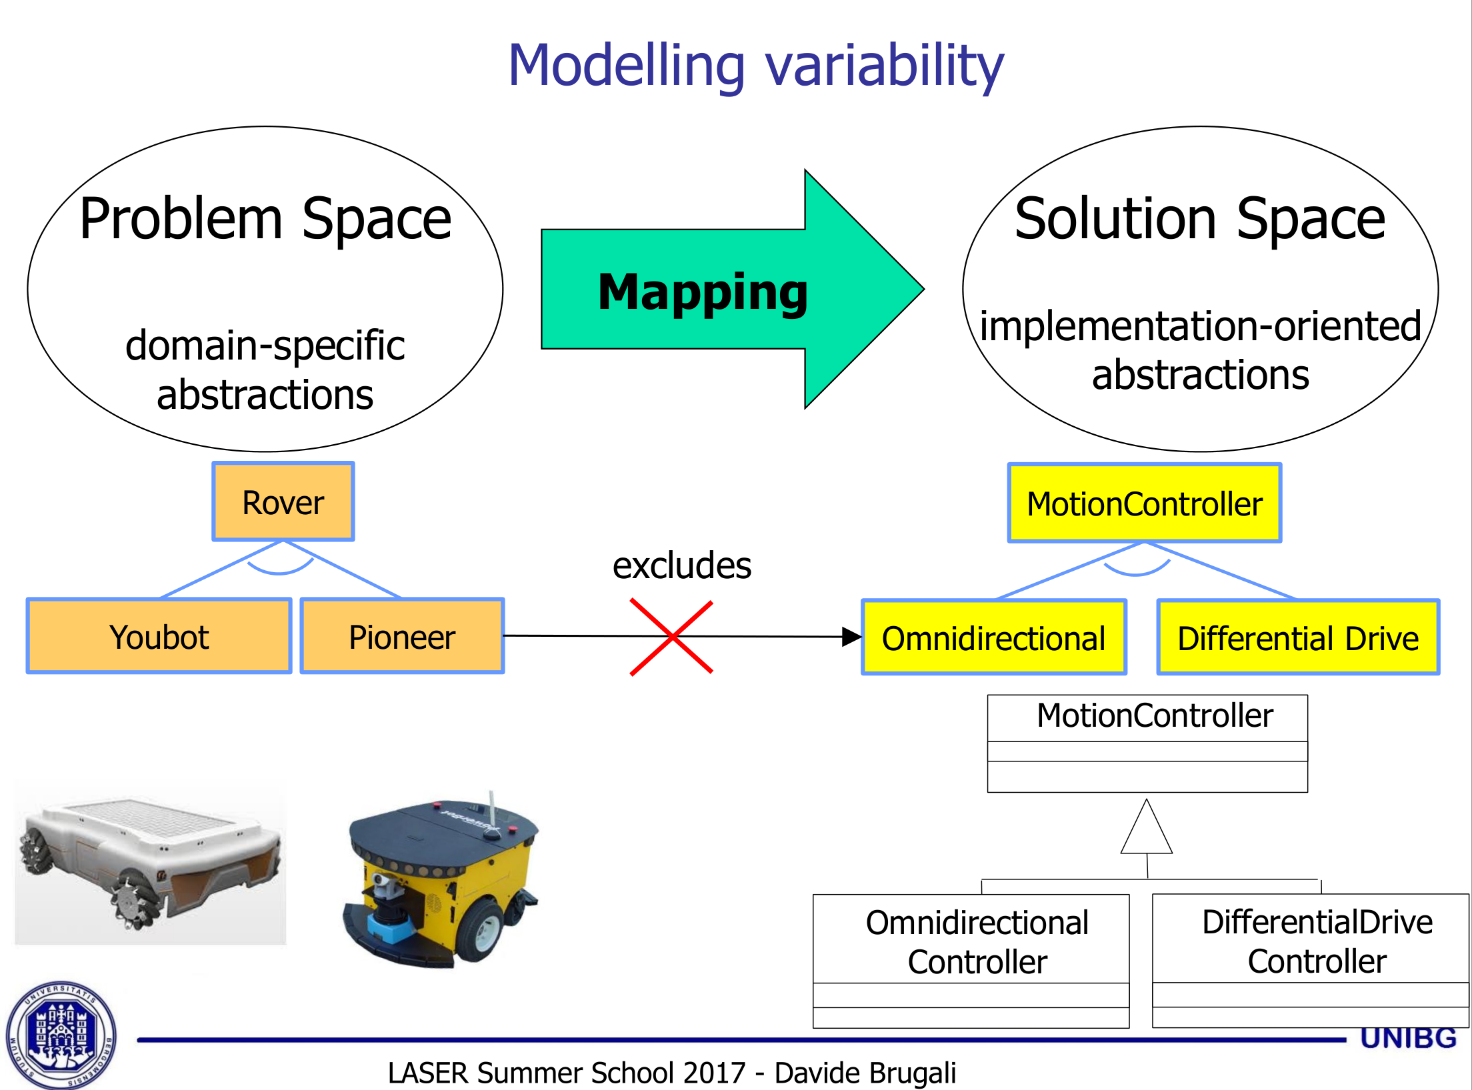
\includegraphics[width=0.9\textwidth]{brugali8.png}
		\end{center}
	\end{frame}

	\begin{frame}
		\begin{center}
			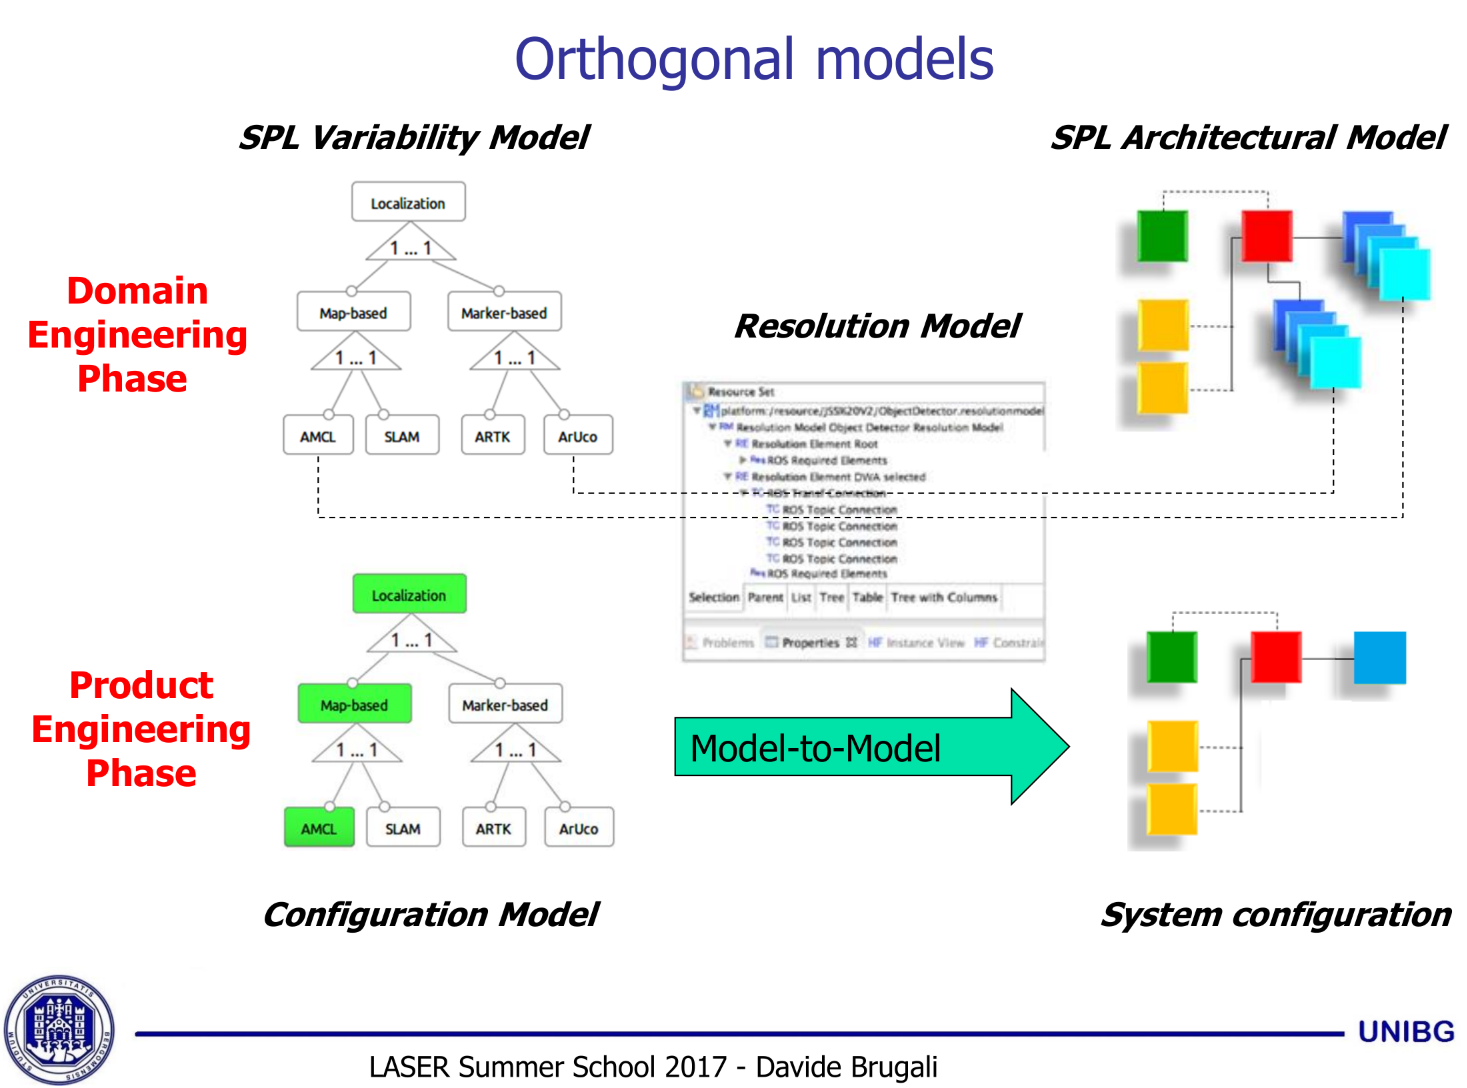
\includegraphics[width=0.9\textwidth]{brugali9.png}
		\end{center}
	\end{frame}

	\begin{frame}
		\begin{center}
			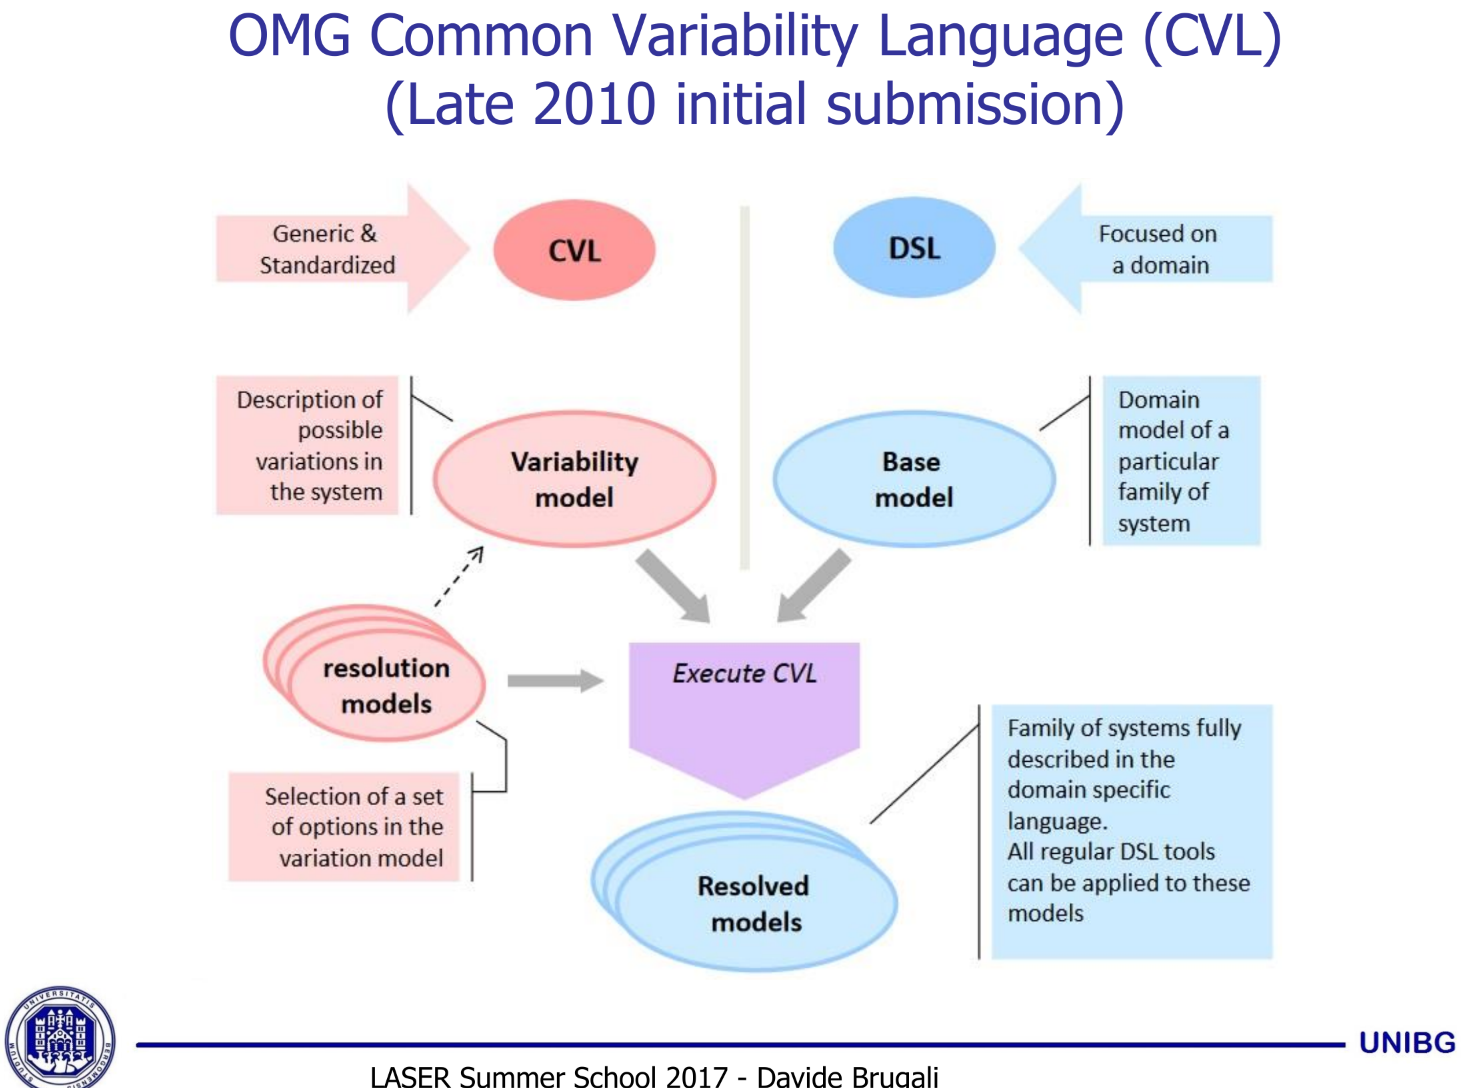
\includegraphics[width=0.9\textwidth]{brugali10.png}
		\end{center}
	\end{frame}

	\begin{frame}
		\begin{center}
			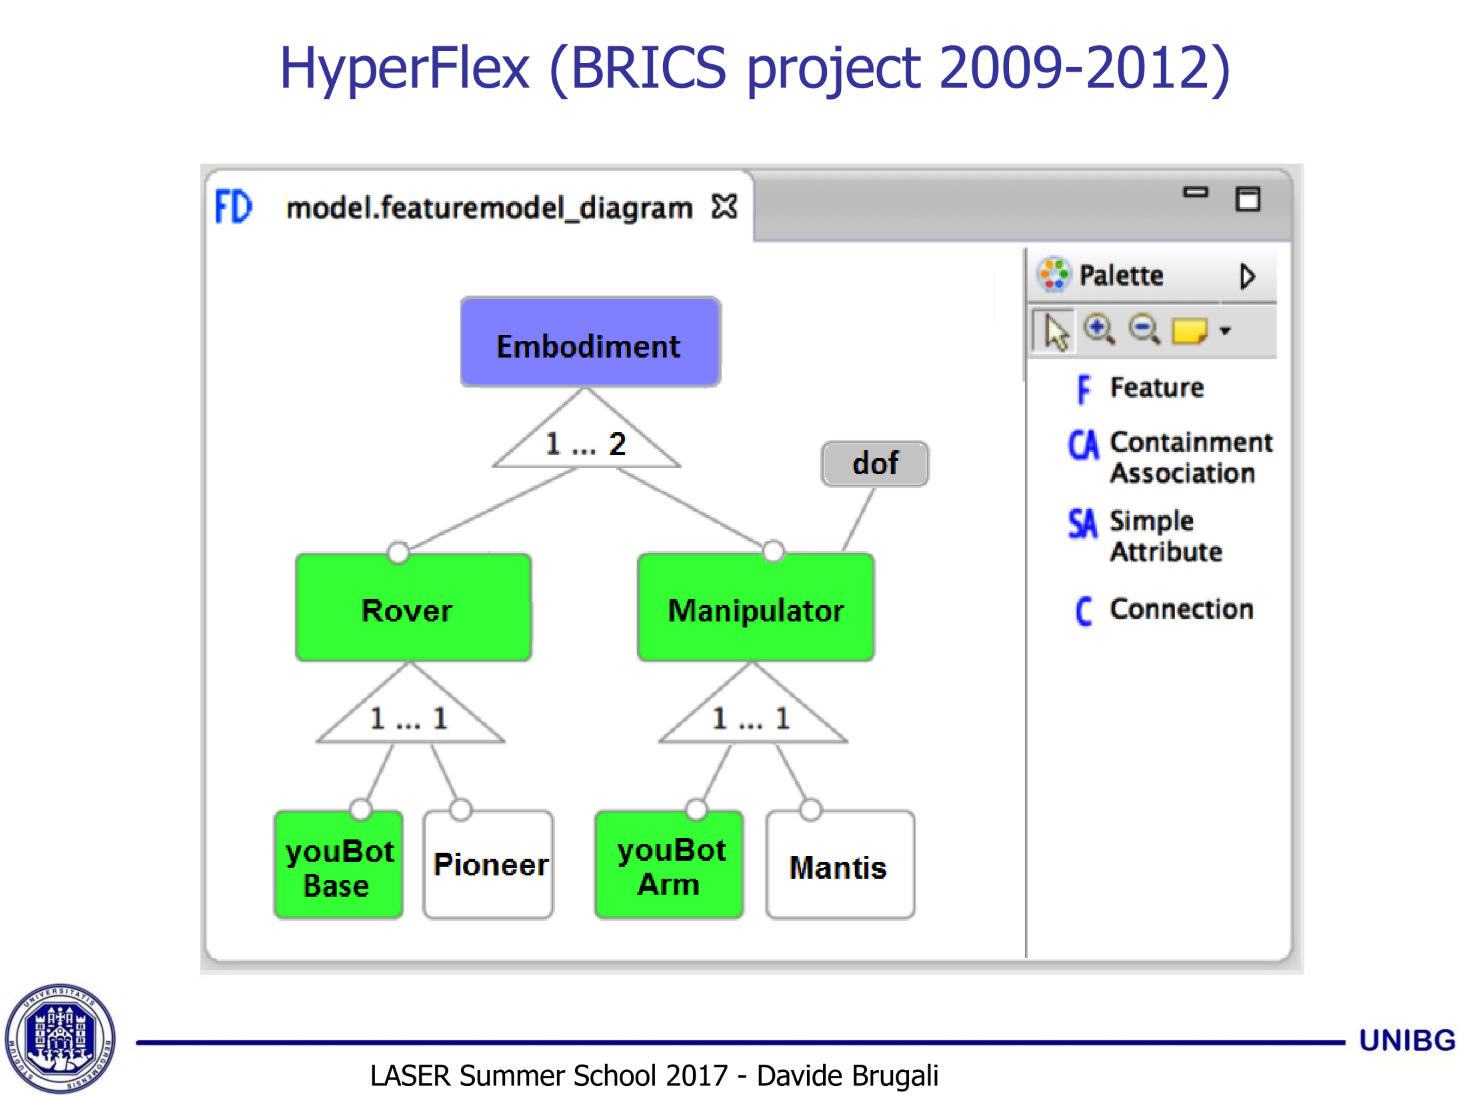
\includegraphics[width=0.9\textwidth]{brugali11.png}
		\end{center}
	\end{frame}

	\begin{frame}
		\begin{center}
			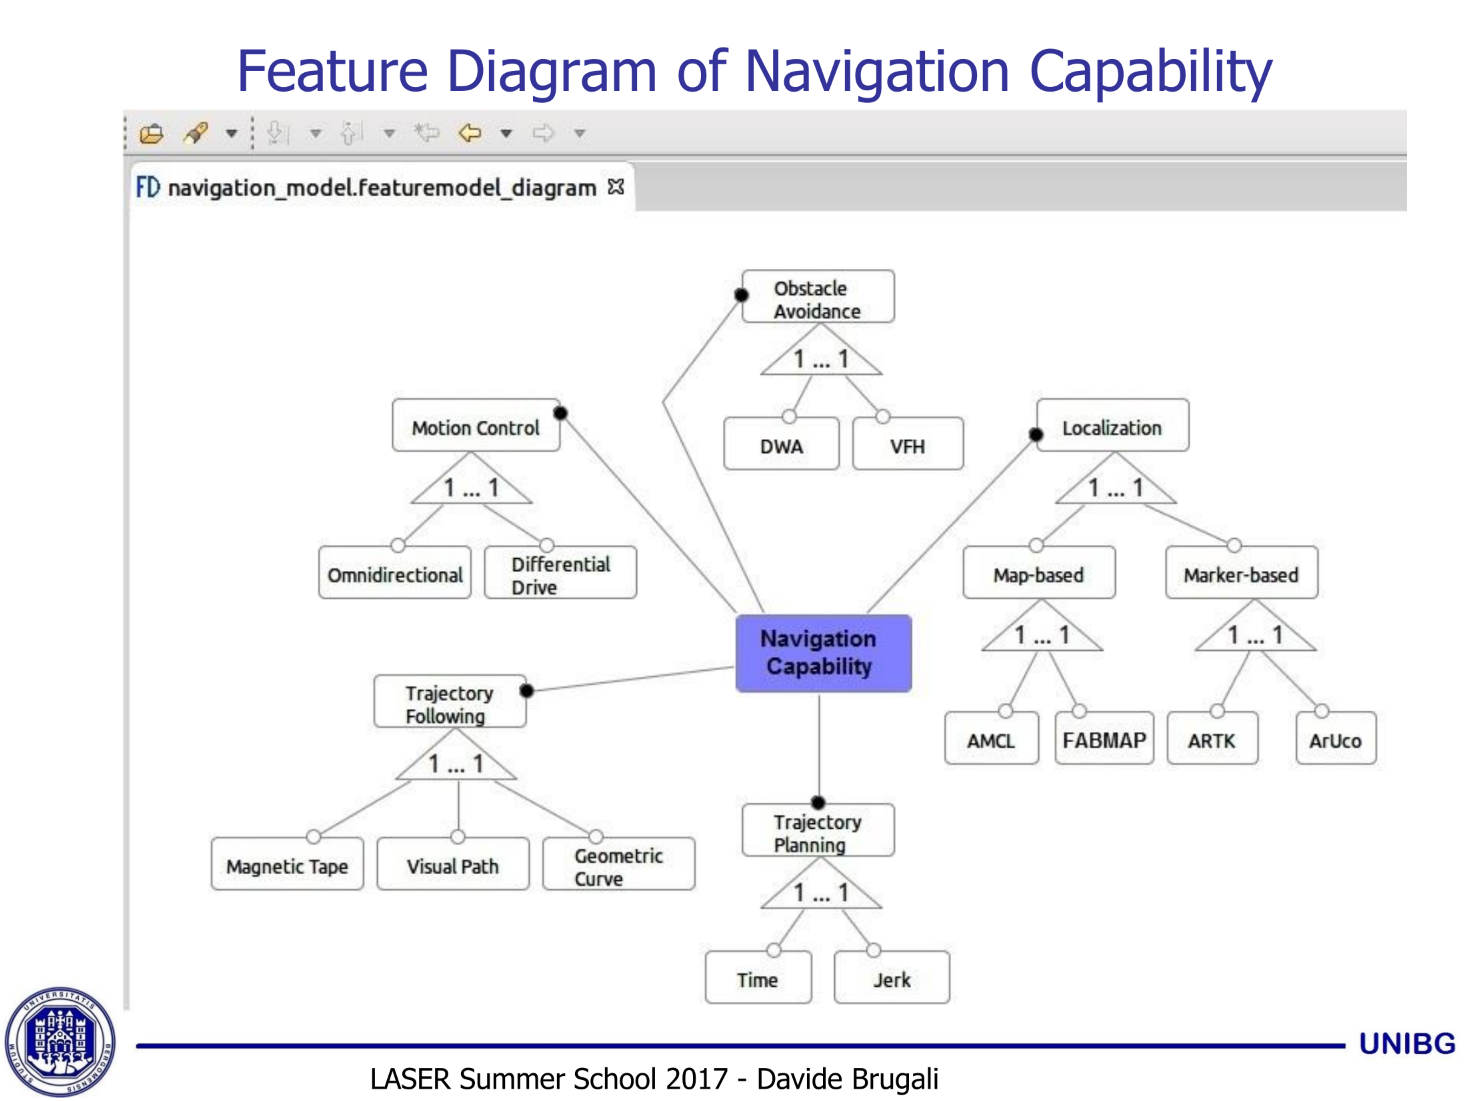
\includegraphics[width=0.9\textwidth]{brugali12.png}
		\end{center}
	\end{frame}

	\begin{frame}
		\begin{center}
			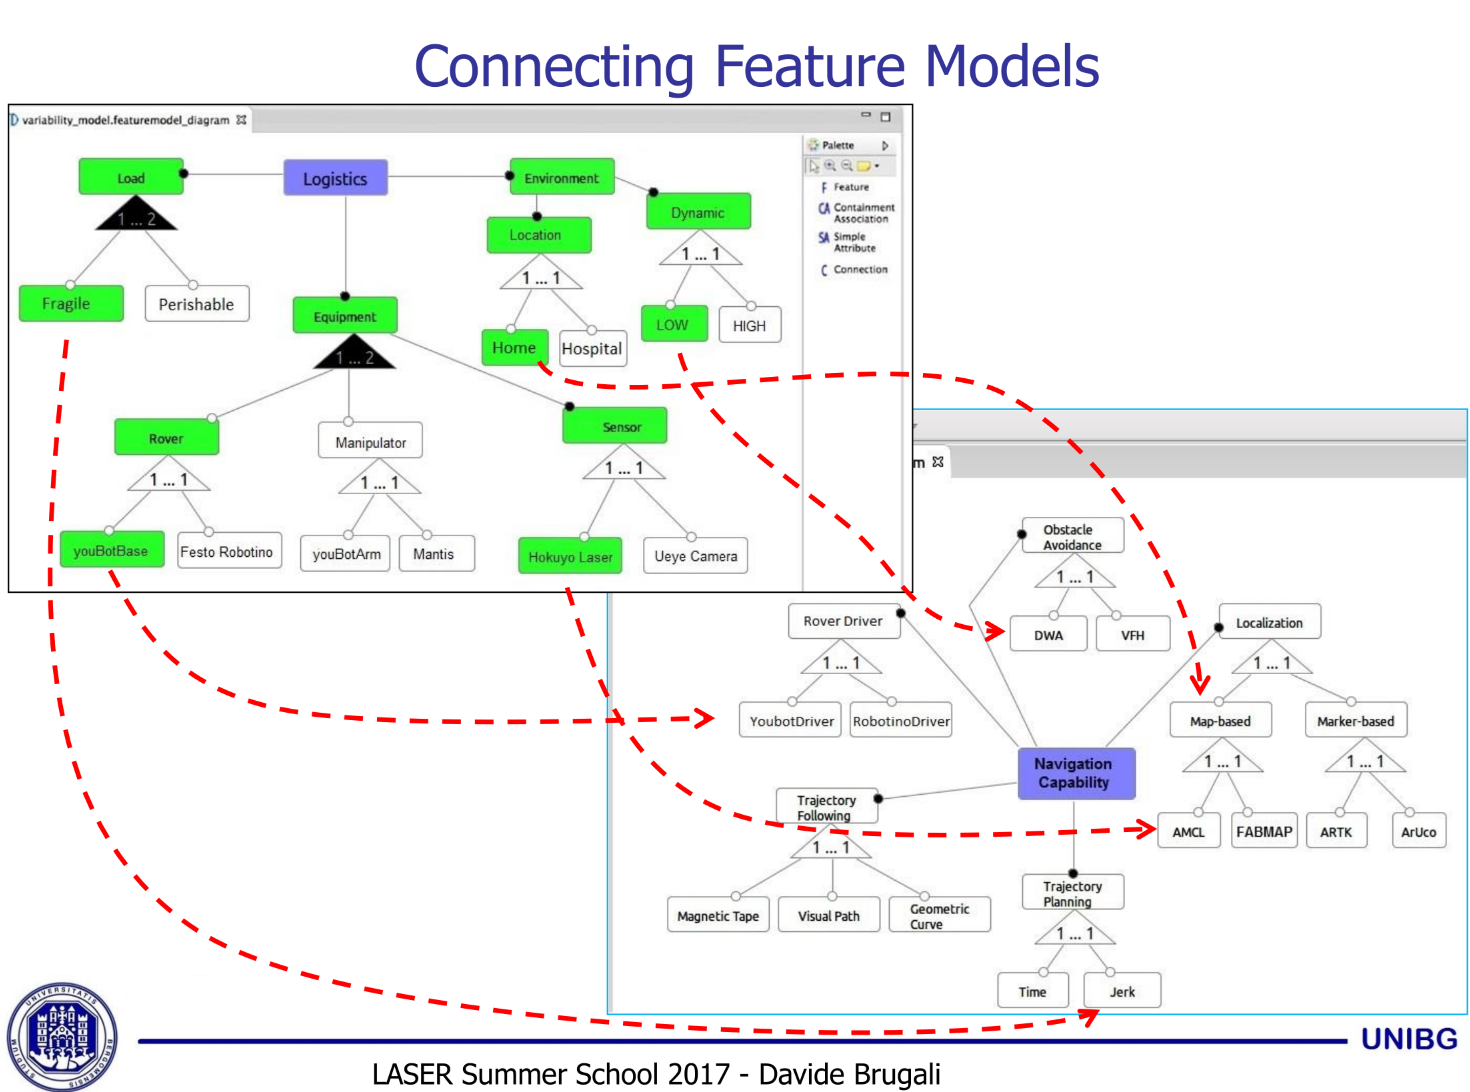
\includegraphics[width=0.9\textwidth]{brugali13.png}
		\end{center}
	\end{frame}

	\begin{frame}
		\begin{center}
			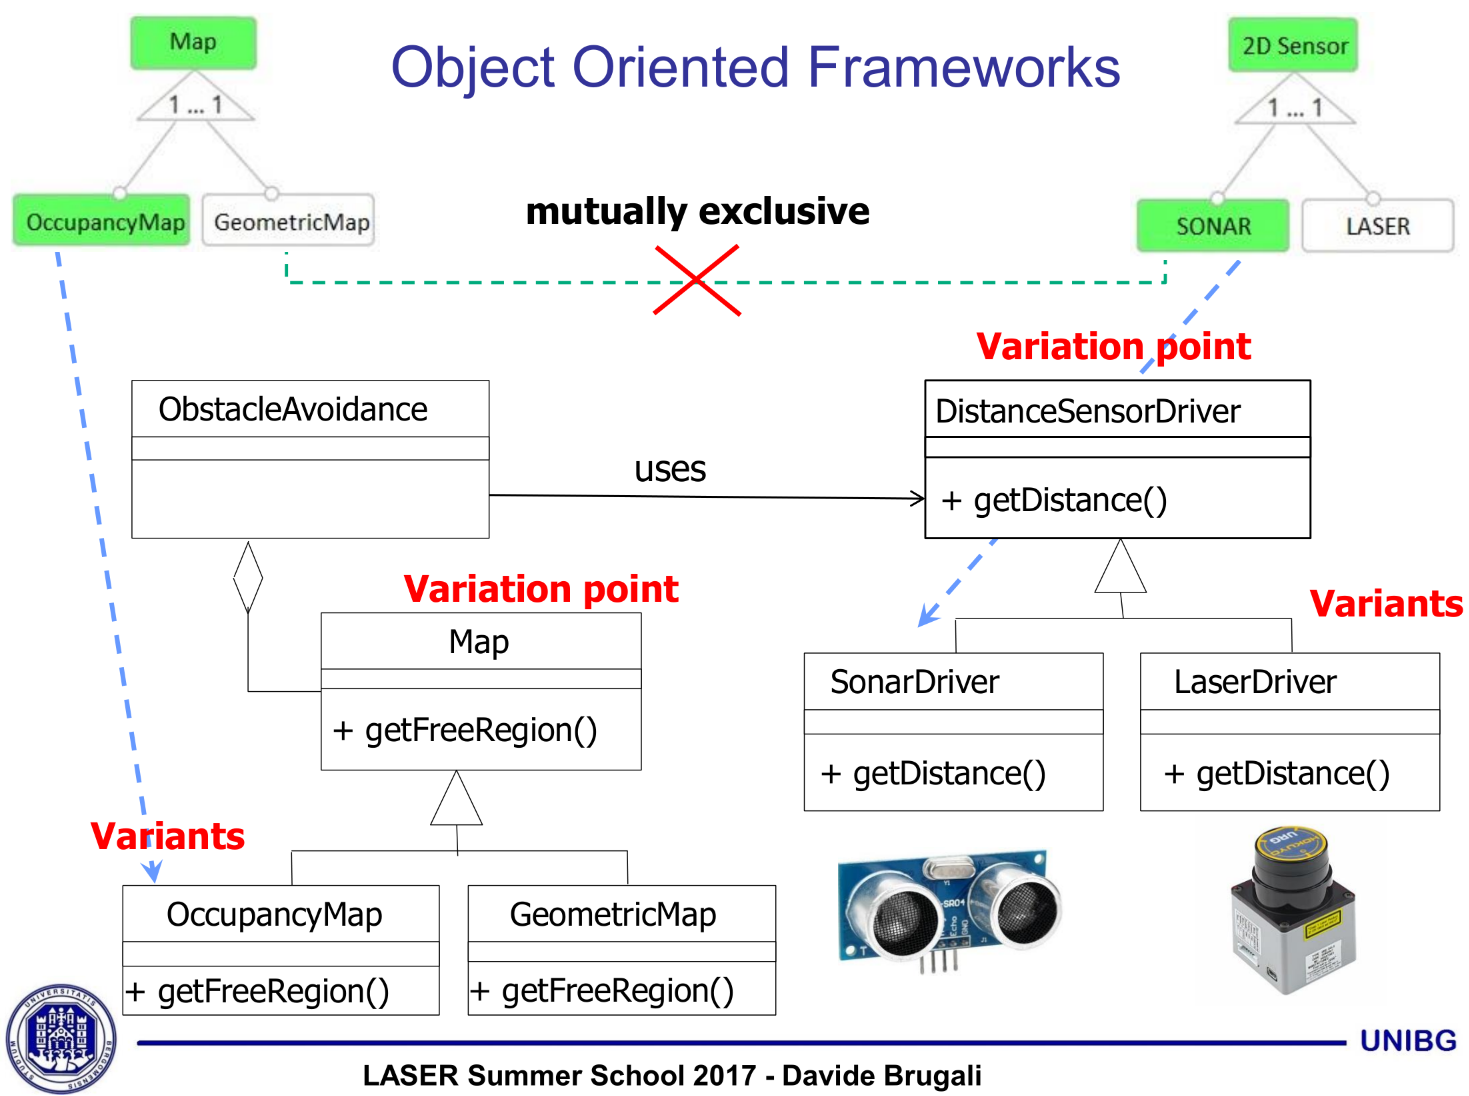
\includegraphics[width=0.9\textwidth]{brugali14.png}
		\end{center}
	\end{frame}

	\begin{frame}
		\begin{center}
			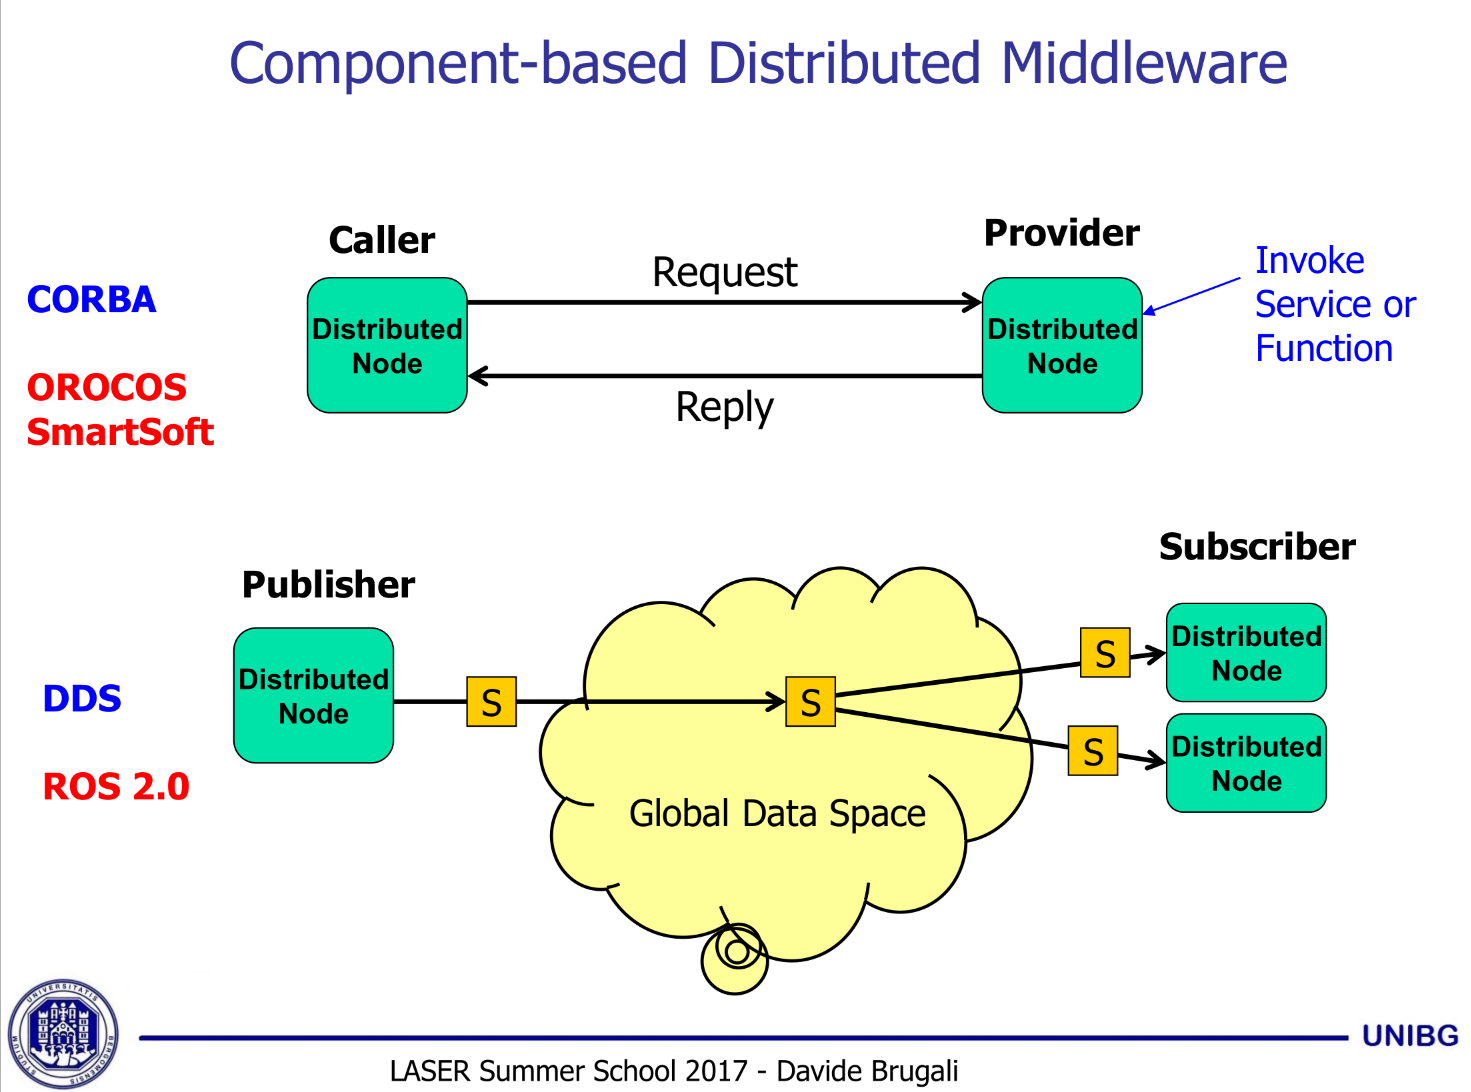
\includegraphics[width=0.9\textwidth]{brugali15.png}
		\end{center}
	\end{frame}

	\begin{frame}
		\begin{center}
			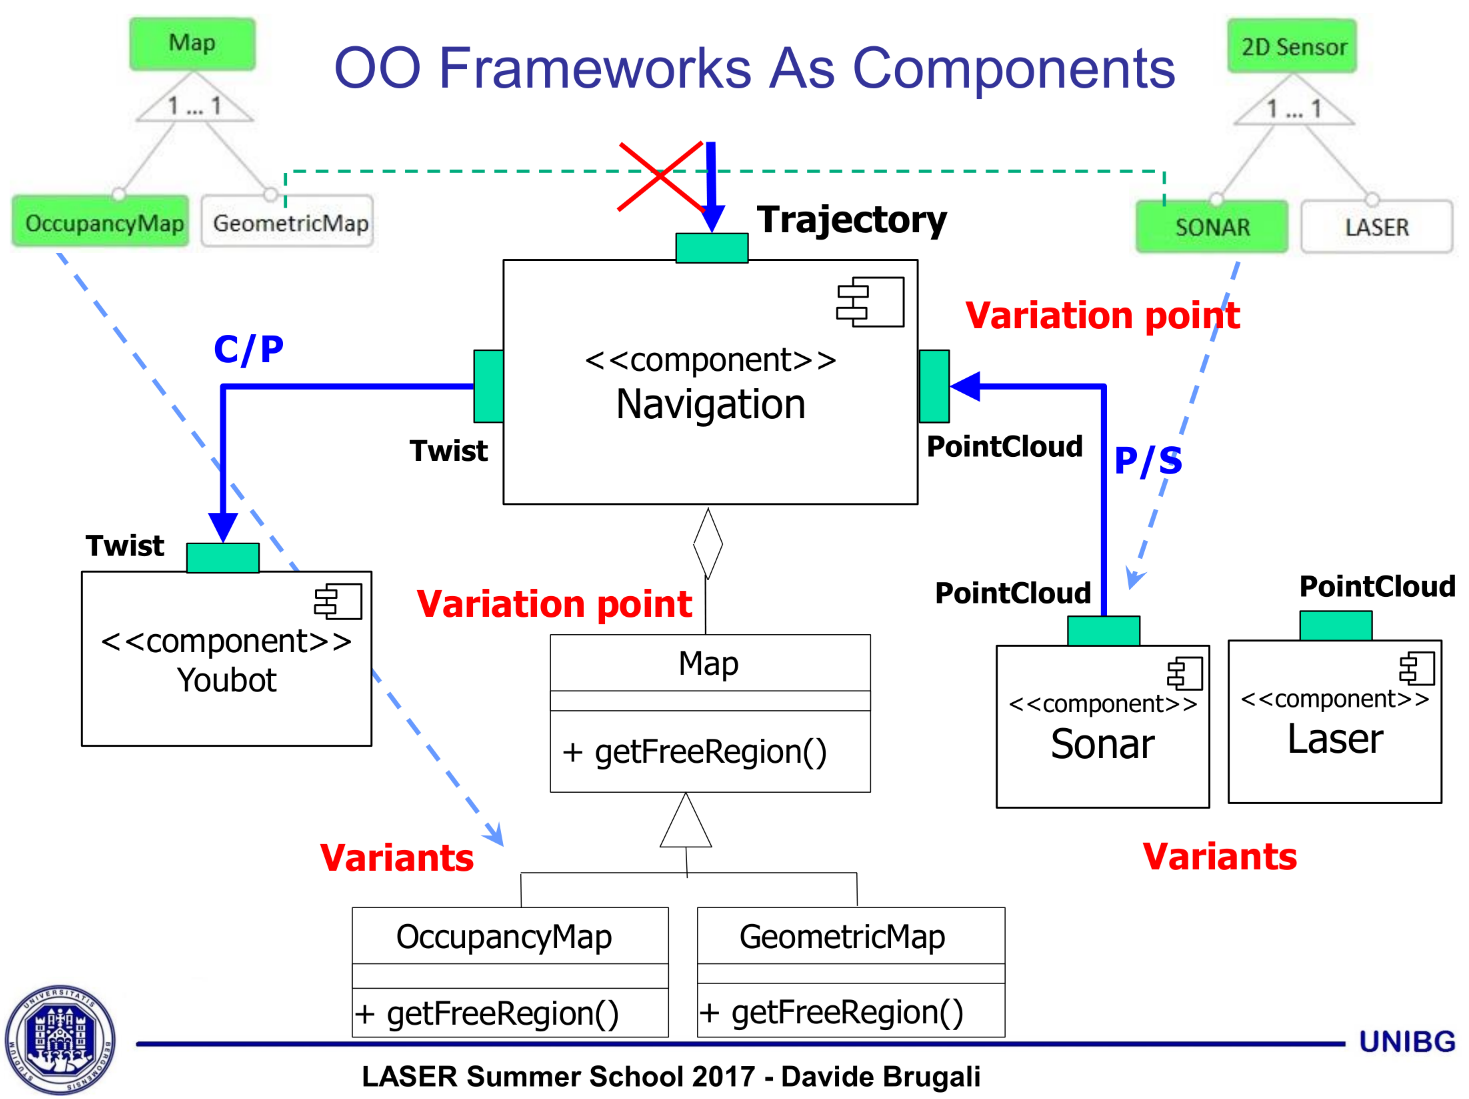
\includegraphics[width=0.9\textwidth]{brugali16.png}
		\end{center}
	\end{frame}

	\begin{frame}
		\begin{center}
			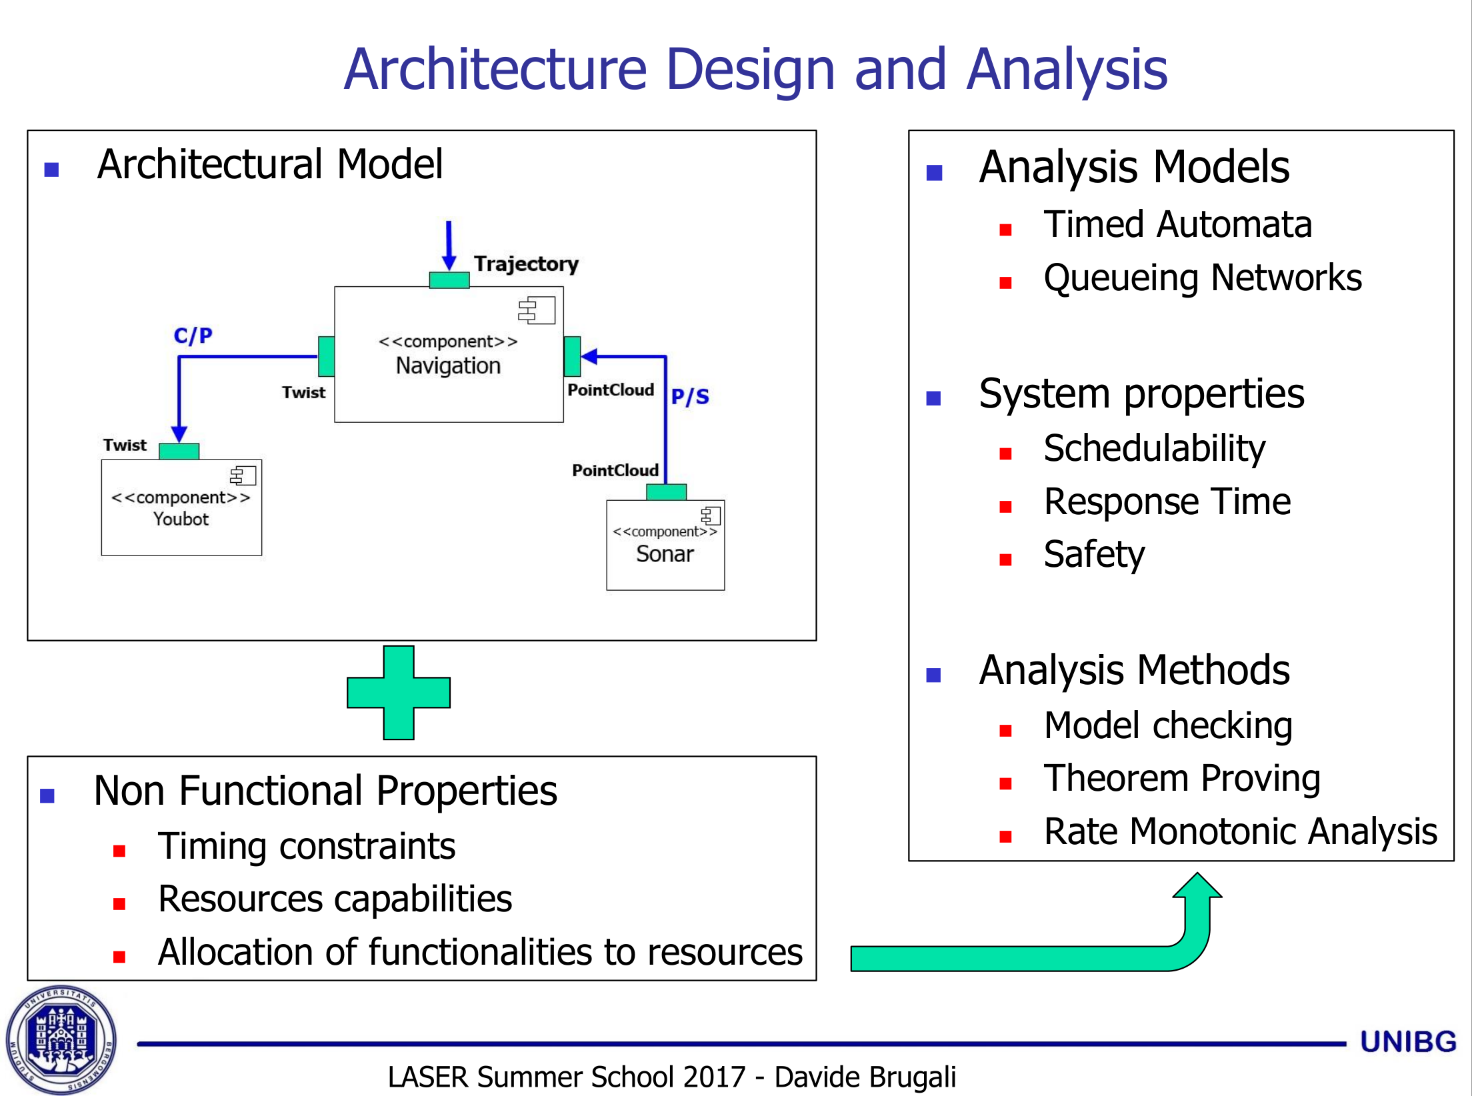
\includegraphics[width=0.9\textwidth]{brugali17.png}
		\end{center}
	\end{frame}

	\begin{frame}
		\begin{center}
			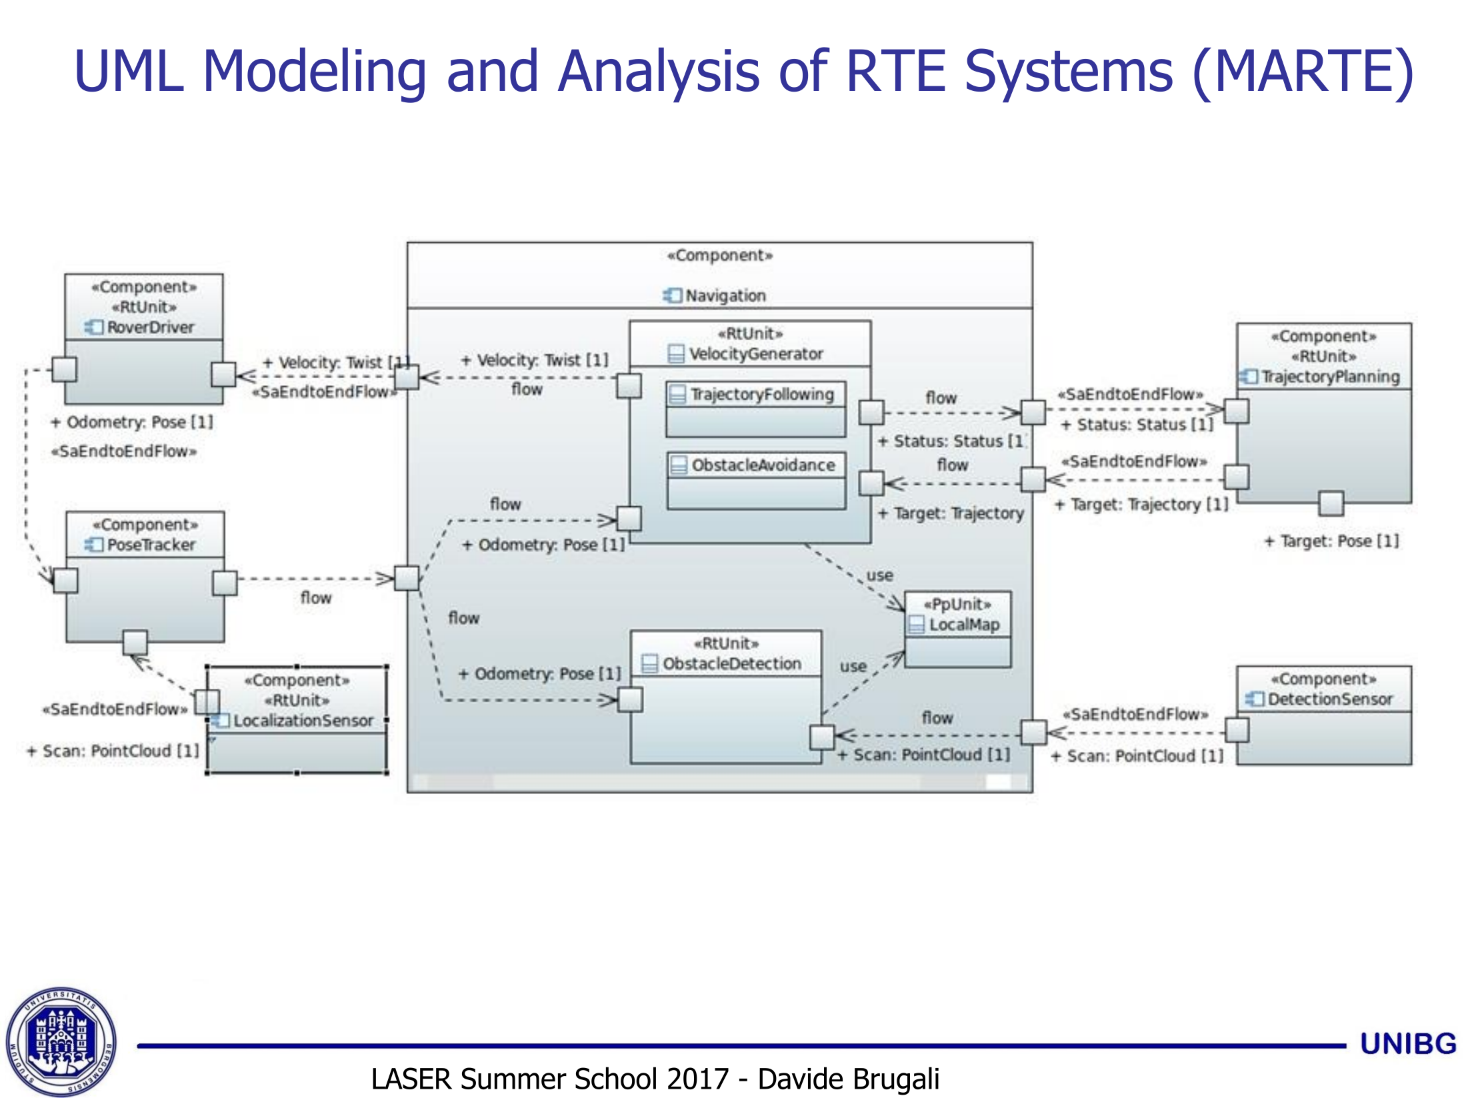
\includegraphics[width=0.9\textwidth]{brugali18.png}
		\end{center}
	\end{frame}

	\begin{frame}
		\begin{center}
			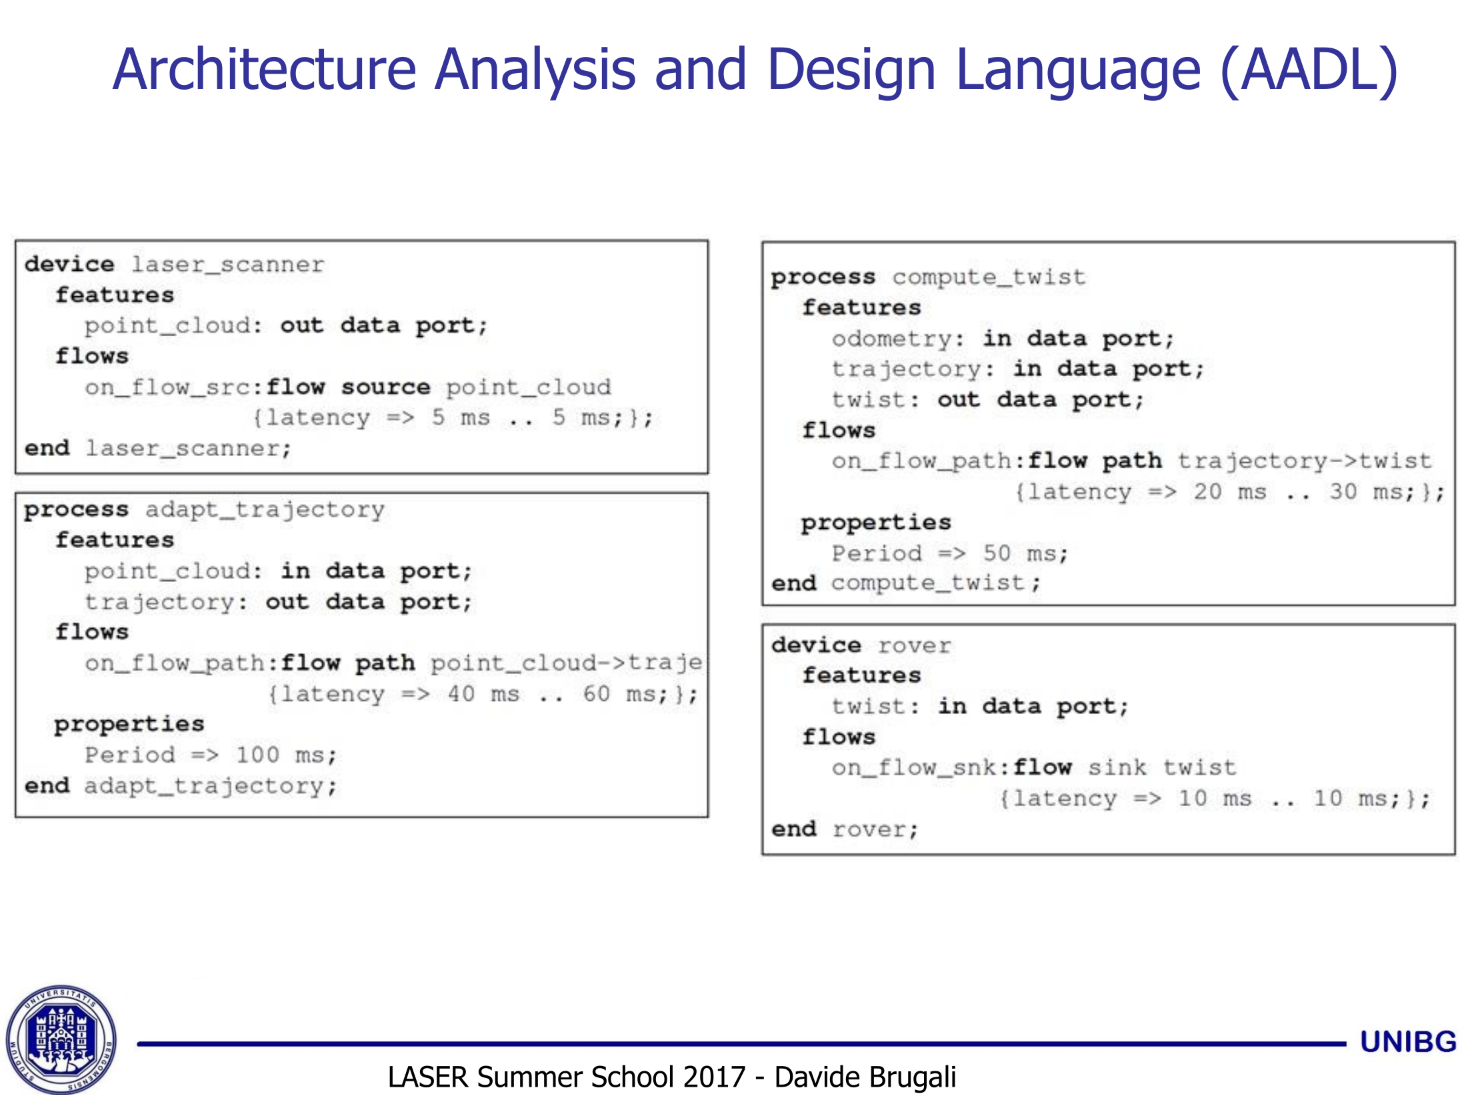
\includegraphics[width=0.9\textwidth]{brugali19.png}
		\end{center}
	\end{frame}

\end{document}

